\chapter{Training Convergence Diagnostics}
\label{app:training_convergence}

This appendix documents the optimization dynamics of the main pipeline configuration (LES-derived placement, $1024$ collocation points, $20\,000$ iterations, seed 42; Table~\ref{tab:main_metrics}), complementing the loss and optimizer description of \S\ref{sec:loss}--\S\ref{sec:optimization}.

Figure~\ref{fig:opt_diagnostics} reports three diagnostics over training. The loss components decrease and plateau. The four GradNorm task weights, initialized at $[1, 0.057, 0.057, 0.01]$ for $[\mathrm{data}, \mathrm{NS}_u, \mathrm{NS}_v, \mathrm{cont}]$, rebalance toward $[1.00, 0.72, 0.79, 0.77]$ as the physics-residual gradients shrink relative to the data term. The Augmented-Lagrangian dual $\lambda_{\rm cont}$ grows monotonically to $0.39$ while the mean-squared continuity residual EMA $\tilde{C}_{\rm ema}$ relaxes toward zero, confirming that the continuity constraint is actively enforced through the dual ascent of \S\ref{subsec:al_cont} rather than only penalized.

\begin{figure}[!htbp]
    \centering
    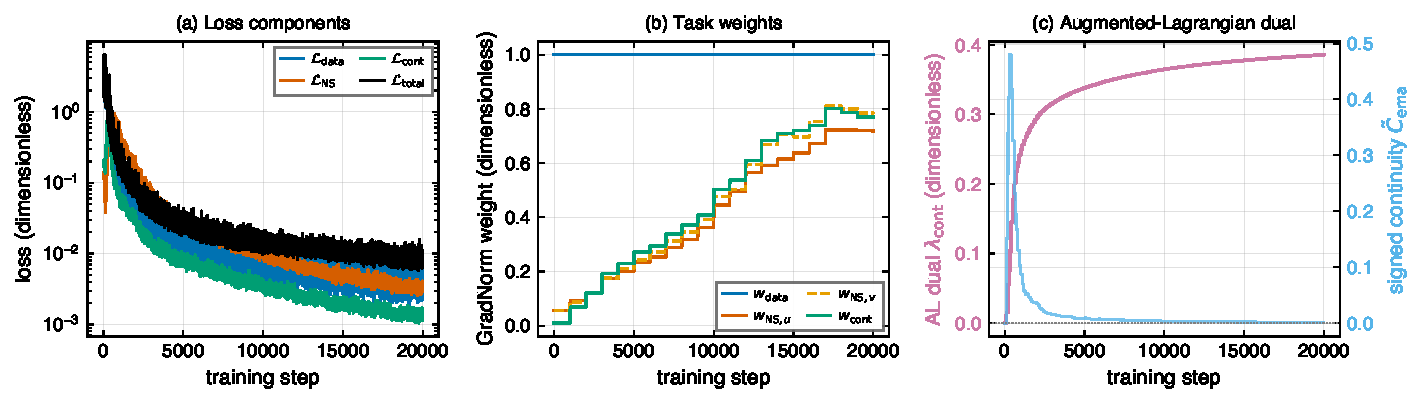
\includegraphics[width=\linewidth]{figures/results/optimization_diagnostics.pdf}
    \caption{Training convergence diagnostics for the main pipeline (seed 42, $20\,000$ iterations). (a) Loss components (dimensionless) versus training step, log scale. (b) GradNorm task weights (dimensionless) versus training step. (c) Augmented-Lagrangian dual $\lambda_{\rm cont}$ (left axis, dimensionless) and mean-squared continuity residual EMA $\tilde{C}_{\rm ema}$ (right axis) versus training step.}
    \label{fig:opt_diagnostics}
\end{figure}
